\documentclass[twocolumn]{article}

\usepackage{kotex}
\usepackage{graphicx}
\graphicspath{ {./images} }

\begin{document}

\title{Zero shot object detection using a foundation model}
\author{
    학번: 2019320016, 이름: 차주한 \\
    지도교수: 김현우 (서명)}
\date{2022.3.28}
\maketitle

\section{Problem (문제 정의)}
In order to make life-saving drone, object detection model is needed to find an object and determine whether it is a person or not.
Especially in the place like a store, there are many object that can be misclassified to be a person like mannequin, person image in posters or reflected person by glass or mirror.
However many existing models are not trained for this kind of tasks, and it is also hard to train a new model from scratch by collecting new data.
Making a golden labeled dataset is a cumbersome work and training a model from scratch need lots of resources.

Recently, research has been conducted to pre-train the foundation model and then perform classification through zero-shot transfer to downstream tasks.
For example, CLIP(Radford et al. 2021)\cite{radford2021learning} uses pairs of image and natural language that describes an image during pre-training.
It uses natural language as supervision for image to learn image representations and it achieved SOTA in many downstream tasks.

However, for zero-shot transfer to succeed, prompt engineering needs to be also performed.
This is because in zero-shot transfer using CLIP, better performance is achieved when labels are given in the form of natural language rather than just words.
So in order to perform aforementioned task successfully, prompt engineering study on what form of natural language each label should be given.

In addition, the data provided by drone is not static images, but video data captured in real time, so the speed for real-time processing is also important.
The performance difference will increase depending on which vision backbone and which object detection framework is used.
For example, according to Ren et al. 2015\cite{ren2015faster}, when using VGG-16 as vision backbone and Selective Search + Fast R-CNN, the processing speed was only 0.5fps.
However, changing the object detection framework to RPN + Fast R-CNN increased processing speed up to 5 fps.
Furthermore, if ZF net is used as vision backbone, the processing speed incresead to 17 fps.
So it is essential to study whhich vision backbone and object detection framework will to use.

\section{Approach (아이디어)}
First, collect data for an aforementioned task and perform zero-shot, few-shot transfer and fine tuning to just classification task and compare which methods performs best.
Then apply some object detection frameworks like R-CNN family, YOLO, DETR etc. and compare performances.

\subsection{Collecting Data}
To collect images for task, I used some publicly available images searched by some keywords.
For example, I searched image with "mannequin in store" to collect mannequin images, because in store, mannequin can be easily found and person or printed person images appear frequently with mannequins in a single shot.
After collected images, I removed some images where mannequin has no head or legs or is synthesized on solid colored background.
One interesting thing in images searched by this keyword is that displayed clothes look like dressed mannequin or person.

\begin{figure*}
    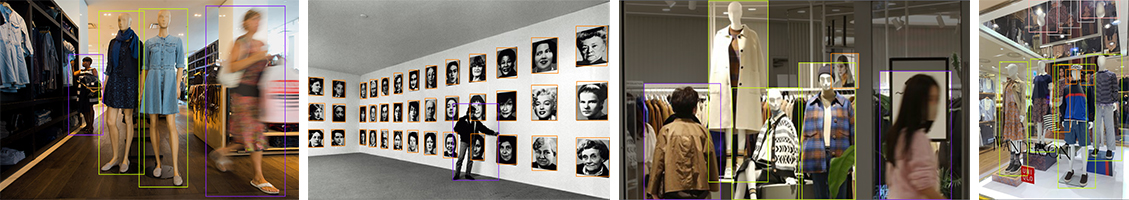
\includegraphics[width=\textwidth]{images/1.jpg}
    \caption{\textbf{Some of collected images.} To test performance of CLIP's classification task to collected images, I cropped the image near bounding box and fed to model.}
\end{figure*}

To find images that contain poster with person image, I used "photo exhibition" keyword and eliminated images that are not portrait exhibition.
Originally, I tried to find exact image for task, but there was no enough image that poster is on the wall and there were only poster image itself.

Lastly, to find image of reflected person or mannequin, I used "person(mannequin) reflected by mirror" and "person(mannequin) reflected by glass" and somewhat similar keywords, because object can be reflected by various objects.

For all images, I removed images where shorter side is smaller than 200px or there is watermark on object that can cause some correlations.

\bibliographystyle{acm}
\bibliography{reference}

\end{document}

